%
\section{Metodi di Machine Learning}
\label{sec:metodi di machine learning}
%

In questa sezione verranno presentate, in maniera descrittiva, le più popolari metodologie di machine learning.\\

\subsection{Iperparametri e Grid Search}
\label{iperparametri e grid search}

Prima di parlare del Grid Search è necessario introdurre il concetto di \textbf{iperparametro}. Come detto nelle sezioni precedenti, un modello di apprendimento è caratterizzato da una serie di parametri che vengono modificati in maniera iterativa in modo da minimizzare la Loss function e, come noto, tale processo avviene attraverso un continuo confronto con il training data set. Quando si parla di iperparametri si intende invece una serie di parametri che caratterizzano il modello implementato che non sono modificati nel processo di addestramento con il training data set ma vengono prestabiliti dall'utente. \\
Chiaramente al variare degli iperparametri cambia anche la qualità del processo di apprendimento del modello e quindi anch'essi devono essere sottoposti ad un processo di ottimizzazione. A questo punto entra in gioco il metodo del Grid Search che è appunto un metodo di ottimizzazione degli iperparametri. \\
Il Grid Search è piuttosto semplice sia da comprendere concettualmente sia da implementare nella pratica; fa parte dei così detti "Brute-Force Search", cioè di quei metodi che si basano sulla sistematica verifica di tutte le possibili soluzioni ad un problema per poi considerare la migliore. Per esempio si consideri il problema di dover cercare i divisori di un numero n: un approccio "Brute-Force" prevedrebbe di considerare tutti i numeri minori di n e verificare quelli per i quali la divisione non dà resto. Questo esempio permette anche di mettere in evidenza il limite principale di tale tipologia di approccio: il numero di possibilità da esplorare può aumentare molto velocemente, soprattutto se si considera un processo multivariato. \\
Tornando ora nello specifico al Grid Search, si consideri un modello caratterizzato da un numero k di iperparametri. Si può definire, in analogia a ciò che è stato fatto con i parametri, un vettore le cui componenti sono appunto gli iperparametri: 
\begin{equation}
\bm{\mu} = (\mu_1,...,\mu_k)
\end{equation}
Tale vettore apparterrà ovviamente ad uno spazio k-dimensionale, sul quale può essere costruita una griglia i cui nodi corrispondono a particolari combinazioni degli iperparametri. \\
A questo punto si può avviare l'apprendimento del modello per ogni particolare configurazione degli iperparametri ed ottenere un valore per la Loss function. Si arriva allora ad avere una valore della Loss per ogni nodo della griglia e quindi basta considerare quello per il quale la Loss è minore, ottenendo la miglior configurazione degli iperparametri. \\
In Figura ~\ref{fig:Grid Search} nella pagina seguente è riportato per chiarezza un esempio visivo dell'esito di un processo di ottimizzazione degli iperparametri attraverso il metodo Grid Search.

\begin{figure}[h!]
	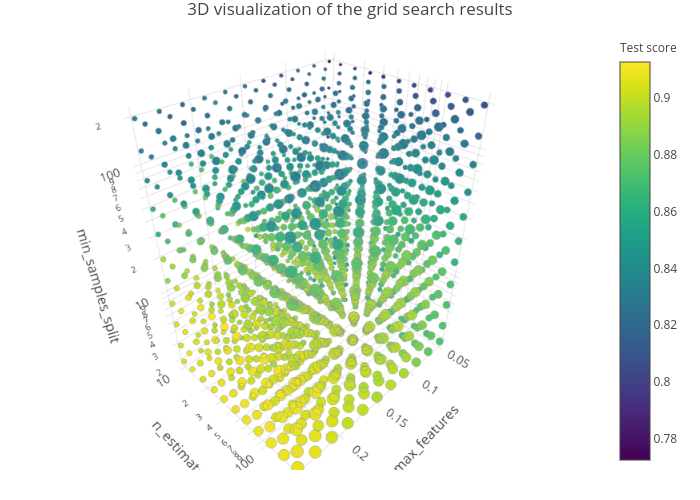
\includegraphics[width=\linewidth]{figs/Grid_immagine.png}
	\caption{la figura illustra visivamente l'esito di un processo di ottimizzazione degli iperparametri attraverso il metodo Grid Search (~\cite{knuthwebsite})}
	\label{fig:Grid Search}
\end{figure}
\newpage 

Come accennato precedentemente, man mano che aumenta la complessità del modello è molto probabile che aumenti il numero degli iperparametri e quindi la dimensionalità dello spazio introdotto precedentemente; ciò implica l'aumento considerevole del numero di configurazioni degli iperparametri da esplorare attraverso il Grid Search e quindi il tempo necessario per concludere l'ottimizzazione.\\
E' possibile ovviare parzialmente a questo problema attraverso il Random Grid Search (RGS), dove non sono considerati tutti i nodi della griglia, ma solo una loro parte selezionata in maniera casuale secondo una particolare distribuzione (ciò permette anche di tener conto di conoscenze pregresse). \\
Come esempio si riporta un problema molto comune nel campo della fisica delle alte energie, ovvero la separazione del segnale dal fondo. Si consideri, per semplicità, un processo bi-variato $\textbf{x} = (x_1,x_2)$ dove, per raggiungere l'obiettivo prefissato di separazione fra segnale e fondo, è necessario applicare un così detto taglio, ovvero stabilire un punto nello spazio bidimensionale $\textbf{P} = (P_1,P_2)$ che permette di dividere lo stesso in due porzioni, come illustrato in Figura ~\ref{fig:grid_example}.\\
Chiaramente la scelta di tale punto deve essere fatta in modo da ottimizzare la separazione segnale-fondo e quindi si può utilizzare il metodo del Grid Search o meglio il RGS per le ragioni presentate precedentemente. 

\begin{figure}[h!]
	\centering
	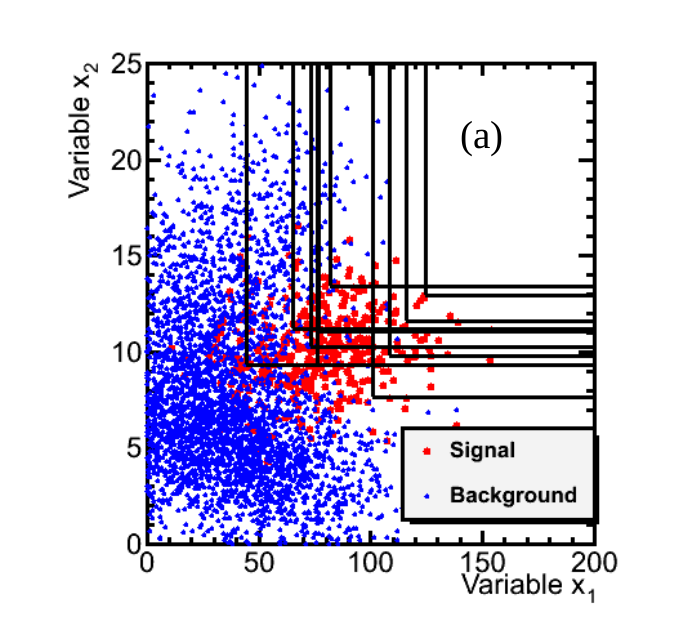
\includegraphics[width=0.85\textwidth]{figs/Grid_example.png}
	\caption{risultato grafico di un processo di Random Grid Search per la separazione del segnale dal fondo in un processo bi-variato. L'immagine è presa da \cite{Metodi_multivariati}.}
	\label{fig:grid_example}
\end{figure}
\newpage

Come si evince dalla figura, un notevole limite del Grid search in questo caso particolare (e della sua variante RDG) sta nell'essere vincolati a dei tagli paralleli agli assi e quindi ci si trova difronte ad un risultato piuttosto limitante. Si possono introdurre a questo punto i Metodi Lineari, continuando a seguire il percorso già accennato in precedenza, ovvero partire dal metodo concettualmente e praticamente più semplice ma meno efficiente per poi salire mano mano di complessità e di efficienza.\\

\newpage

\subsection{Analisi discriminante lineare}
\label{metodi lineari e discriminante di Fisher}

Come detto nella sezione precedente, il GS ed il RDG possono essere utilizzati per la separazione del segnale dal fondo ma hanno dei limiti piuttosto considerevoli che sono già stati illustrati. L'analisi discriminante è un metodo che permette di raggiungere lo stesso obiettivo di separazione, ma in modo più efficiente. \\
L'analisi discriminante si definisce lineare quando la funzione classificatrice è, appunto, lineare. \\
Si immagini di avere a disposizione un determinato set di eventi in input $\textbf{x}_\textbf{i}$, ciascuno caratterizzato da un numero n di variabili (spazio n-dimensionale) e di volerli ripartire fra segnale e fondo.\\
Si definisce la funzione discriminante lineare nel seguente modo:
\begin{equation}
D(x_1 , x_2 , ... , x_n) = c_0 + c_1x_1 + ... +c_nx_n = c_0 + \sum_{i=0}^{n} c_ix_i 
\end{equation}
quindi come una combinazione lineare delle componenti del vettore che rappresenta l'evento; il valore assunto dalla funzione per ogni singolo evento ne permette la separazione nelle due classi (nel presente caso segnale e fondo), utilizzando un valore di riferimento $D_0$. \\
A questo punto l'obiettivo è quello di massimizzare la distanza fra le due classi, ovvero rendere massima la differenza dei valori assunti dalla funzione $D(\textbf{x})$ fra gli eventi appartenenti al fondo e quelli relativi al segnale. \\
Un esempio di questo approccio è il metodo proposto da Fisher: si consideri un campione di eventi appartenenti al segnale e se ne definisca la media $\bm\mu_\textbf{s}$ e la deviazione standard $\sigma_s$ ed un campione appartenente al fondo, definendo anche qui la media $\bm\mu_\textbf{f}$ e la deviazione standard $\sigma_f$. A questo punto la migliore configurazione dei parametri è quella che massimizza la seguente funzione: 
\begin{equation}
F(\textbf{c}) = \frac{(\bm\mu_\textbf{s} - \bm\mu_\textbf{f})^2}{\sigma_s^2 + \sigma_f^2}
\end{equation}

